\subsection{Sparse-overlapping-sets (SOS) {\lasso}}
\subsubsection{Concepts and assumptions}
The multivariate methods we have considered so far lie at two poles with regard to their assumptions. The searchlight method assumes both localization of signal within individuals and consistency of localization across individuals. Regularized regression discards both assumptions, allowing for the possibility that representations of interest are arbitrarily situated within individuals, in completely different ways across individuals. From the PDP view of representation, the former assumptions seem too restrictive, while the latter assumptions seem too loose. If we believe that all human beings share the same gross neuroanatomical structure, then it seems reasonable to suppose {\em some degree} of localization within individuals and some degree of consistency in location across individuals. Within individuals we might assume that, if a given unit is important for representation, there is a good chance that some other units in the general vicinity are also important. Such an assumption could be adopted without further requiring that {\em all} neighboring units are important (univariate assumption 1), or that {\em only} neighboring units contain sufficient information for the representation (searchlight assumption 1). Likewise we might assume that, if a set of voxels contribute to a representation in individual A, then signal-carrying voxels are likely to be found in the same general anatomical vicinity in individual B. Such an assumption could be adopted without requiring that the location of the interesting information is very precisely aligned, or that the location contains useful information in the great majority of individuals (assumption 3 for univariate and searchlight).

With these intuitions in mind, the final method we consider is the {\soslasso} ({\soslassofull}, recently introduced by  \citeA{raoNIPS}). {\soslasso} is a variant of {\lasso} that allows for evaluation of a range of hypotheses regarding localization within and across individuals. It adopts a central and intuitive assumption from {\em multi-task learning} \cite{Caruana97}: if a set of learning tasks are related, then their solutions will also be related. In this case, each ``task'' is to find the neural activation pattern associated with a particular mental state in a single individual. In contrast to {\lasso}, we assume that the solutions across individuals are related: finding useful information in one individual gives us clues about where to look in another. The loose assumptions about localization within and across individuals can be built into a single optimization function that considers all subjects at once.

To achieve this, the voxels in the datasets from every individual are assigned to {\em sets}. Within an individual, voxels belonging to a given set are related to one another in some way--for instance, if the sets are defined by anatomical proximity, voxels within a set will all be near one another. Across individuals sets are aligned, so that voxels in {\em Set 1} for individual 1 are related to voxels in {\em Set 1} of individuals 2 through {\em n}. If sets are defined by anatomical proximity, then voxels in Set 1 will be localized similarly across subjects. The optimization then operates over all subject datasets simultaneously, minimizing an objective function that prefers solutions in which selected voxels belong to as few sets as possible. The end result is a solution that is unique for each dataset (i.e., each individual), but with the selected voxels tending to belong to the same sets within and across individuals. 

Before considering the objective function itself, it is useful to consider how voxels are assigned to sets. Such assignments are made {\em a priori}, and can in principle be guided by any hypothesis about how voxel sets are best grouped. For instance, sets might be determined by an anatomical segmentation, a previous analysis, a literature review, or any other prior knowledge. Importantly, however, set assignment can also be done in a relatively theory-neutral way: a volume can be split into a collection of {\em overlapping} sets of fixed size and degree of overlap, with each voxel belonging to multiple overlapping sets. On this approach, the voxels for each individual are first projected into a common anatomical reference space (without blurring). The space is divided into a 3-dimensional grid and, for each gridpoint, all voxels within radius $r$ are assigned to a given set. Each set thus contains a group of voxels in roughly the same anatomical location across subjects; each voxel belongs to multiple sets; and the sets overlap in the voxels they contain. The sets are analogous to searchlights, but rather than training separate classifiers for each set in each subject, a regularized logistic classifier is trained on all the data together. Because the optimization prefers solutions in which voxels belong to a small number of sets, such an approach will automatically select the particular grouping of voxels within and across individuals that best minimizes the objective. But, because the solutions are unique to each individual, there is no need for all voxels within a set to be selected or to receive similar weightings within or across individuals.


% This is tantamount to hypothesizing that the probability of a voxel carrying true signal is higher if it is in the vicinity of other voxels that appear to be informative. Because sets may overlap, it allows for flexible definitions of similarity, and allows one to avoid committing to a particular structure prematurely. This way of defining sets bares some similarity to the searchlight method. The critical difference is that a searchlight analysis handles each localized region in isolation of all others, while {\soslasso} performs a single optimization over all sets at once to train a single logistic classifier.

%The final method we consider is a variant of {\lasso}, the Sparse Overlapping Sets Lasso ({\soslasso}; \citeNP{raoNIPS,raoML}), which assumes a loose degree of localization within individuals and a loose degree of consistency in location across individuals. {\soslasso} employs {\em multi-task learning} \cite{Caruana97}, which makes an intuitive assumption: if a set of learning tasks are related, then their solutions will also be related. In this case, each ``task'' is to find the representation associated with a particular mental state in a single individual. In contrast to {\lasso}, we assume that the solutions across individuals are related: finding useful information in one individual gives us clues about where to look in another. The loose assumptions about localization within and across individuals can be built into a single optimization function that considers all subjects at once. The voxels for each individual are first projected into a common anatomical reference space (without blurring). The space is divided into a 3-dimensional grid and, for each gridpoint, all voxels within radius $r$ are grouped together in a $set$. Each set thus contains a group of voxels in roughly the same anatomical location across subjects. Each voxel belongs to multiple sets, and the sets overlap in the voxels they contain. The sets are analogous to searchlights, but rather than training separate classifiers for each set in each subject, a regularized logistic classifier is trained on all the data together. 

With that conceptual grounding, we can consider the {\soslasso} regularization penalty:

\begin{align}
h(\mathbf{W},\mathbf{S}) = \sum_{s}\left(  \alpha \sqrt{\sum_{i} \mathbf{W}_{si}^2} + (1-\alpha) \sum_{i} |\mathbf{W}_{si}| \right) 
\end{align}

%TR: I changed the G to S above since we are now calling these Sets rather than Groups.

The function has two terms, $\sqrt{\sum{\mathbf{W}^2_{si}}}$ and $\sum{|\mathbf{W}_{si}|}$, which are embedded in a loop that sums over sets. The second term is simply the {\lasso} penalty from Equation \ref{eq.lasso}, computed separately for each set and summed over all sets. The first term, which we will refer to as the {\em set penalty}, takes the root of the squared coefficients summed over units within each set. $\alpha$ is a mixing parameter that determines the weight given to each of these two terms. When $\alpha=0$, the set penalty is not applied and {\soslasso} effectively reduces to {\lasso}. When $\alpha$ is non-zero, however, the penalty behaves differently, preferring solutions where the non-zero coefficients (i.e., the selected voxels) all appear in the same overlapping sets---that is, when they tend to be in similar anatomical locations.

\begin{center}
	\textbf{---Figure \ref{fig.soslossex} about here---}
\end{center}

\begin{figure}
	\centering
	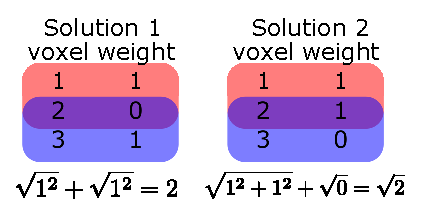
\includegraphics[width=0.95\textwidth]{figures/soslasso_loss_example.eps}
	\caption{A schematic laying out two hypothetical solutions, and the {\em set penalty} they incur. The set penalty is one of the components of the {\soslasso} regularizer. Note that in cases of overlap, the weight will be accounted for only once, as belonging to the set in which it increases the penalty by the smallest amount. In other words, {\soslasso} will consolidate weights into as few groups as possible.}
	\label{fig.soslossex} 
\end{figure}

To understand how this preference is realized, we can compute the penalty associated with two competing solutions in a very simple case, diagrammed in Figure \ref{fig.soslossex}. Consider a 1-dimensional brain with 3 voxels. Voxels 1 and 2 are assigned to {\em Set 1}, and voxels 2 and 3 are assigned to {\em Set 2}. In the first solution, let voxels 1 and 3 be assigned a value of $+1$, and voxel 2 a value of $0$. The set penalty $\sqrt{\sum{\mathbf{W}^2_{gi}}}$ evaluates simply to $\sqrt{1^2} + \sqrt{1^2}=2$, because the voxels are in different sets. In a second solution, let voxels 1 and 2 be assigned a value of $+1$ and voxel 3 a value of $0$. This time, the penalty evaluates to $\sqrt{1^2+1^2}=\sqrt{2}$, because the voxels are in the same set. Because the set penalty takes the root of the sum of squares across voxels in the set, the assignment of a +1 value to 2 of the 3 voxels produces a larger cost when the coefficients are placed on voxels from different sets. 

There is a wrinkle here, of course: voxel 2 also exists in {\em Set 2}. {\soslasso} avoids double counting by applying each weight only where it is least expensive.  In the current case, if we consider the weight assigned to voxel 2 as part of {\em Set 2}, it ``costs'' $1$ penalty unit. If we consider it as part of {\em Set 1} it only costs $\sqrt{2}/2=0.707$ penalty units. In principle the total weight on the voxel could be apportioned across its corresponding sets in any manner; however allocation of the voxel's weight to an otherwise empty group incurs a greater overall penalty, so the optimization ends up placing all of the voxel's weights within sets that also contain other non-zero voxels. In this way the optimization ``knows'' to account for voxel 2 as belonging to {\em Set 1} rather than {\em Set 2}, and does not redundantly penalize the same weight. The further consequence is that the optimization automatically finds sets that contain many signal-carrying voxels if these are present in the data.

%Although the example above considers a single dataset, the concepts readily generalize to multiple datasets. Recall that when assigning voxels to groups, the voxels assigned to {\em Set 1} from different datasets are assumed to be related. In fact, there is only one {\em Set 1}, and all datasets contribute to it. Sets extend across datasets. Thus, when computing the {\em set penalty}, all weights in the set across all datasets, are taken into account.  In fact, if we took our example above and considered each of the active voxels to be from differt datasets the math will work out identically to the single-dataset case. This one mechanism accounts for both of  {\soslasso} 's preferences, localization within individuals and shared structure across individuals.

%TR: I cut the above paragraph b/c I think this is now made clearer in the earlier material

Finally, it is important to note that both the {\em set penalty} and the {\lasso} penalty increase when the magnitude of any weight is increased.  This means that, just as with {\lasso}, solutions that include fewer voxels overall will tend to be preferred. Solutions will be sparse, even within groups. Sets are not selected themselves, but rather voxels are selected from within sets and it is less costly to select multiple voxels from the same set than from different sets.
%To see why this is so, consider a case where there are 9 voxels that each carry important independent information that can best reduce prediction error by receiving a coefficient of +1 in the logistic regression model. Suppose further that the 9 voxels are situated in very different anatomical locations, so that none of them appear in the same group, and that other voxels in each group carry no useful information. In this case, placing a coefficient of +1 on each voxel will incur a cost of 1 for both the {\lasso} term and the set penalty, for a total cost of 18 in each set across the 9 voxels. Now consider what happens if all 9 voxels are near one another so that many sets contain all 9. For each such set, the {\lasso} component of the penalty across the 9 voxels will again be 9, but the set penalty will be smaller: it will be the square root of the sum of squared values over voxels in the set, that is $\sqrt{9}$, or 3. Thus the set penalty per selected voxel is smaller when the predictive voxels appear together in the same set. When the voxels are all very near one another, many sets will contain all 9 voxels, and many more sets will contain some of the 9. Only a few sets will contain just one of the 9 voxels. So the total penalty across all groups will be much smaller than in the case where all 9 voxels are anatomically well separated. In general the set penalty, because it takes the root of the sum of squared coefficients across predictors within groups, is smaller when the predictors are included in similar overlapping sets.

%Note that we have replaced the vector of weights denoted as $\beta$ in Equations \ref{eq.lasso} and \ref{eq.ridge} with a matrix of weights\footnote{{\soslasso} does not only apply to matrices, and can be used for single subject analyses as well. We are describing the multi-task learning case that is most relevant for understanding the applications in this paper.}, $\mathbf{W}$, where rows are voxels and columns are subjects. $\mathbf{G}$ is a matrix where each row is a group, and each column is a is a slot for a voxel index, where a voxel index refers to a row in $\mathbf{W}$. The voxels identified in any given row of $\mathbf{G}$ are assumed to be similar across subjects. What is key to note about the {\soslasso} regularization function is that, when $\alpha>0$, the penalty is less when increasing the weight on two voxels that belong to the same group---within or across subjects---than for increasing the weight on two units from different groups. Consider a simple case: two voxels, each with weight equal to 1. To further simplify, let $\alpha = 1$ to drop the second component of the penalty. If the voxels are in the same group, the function simplifies to $\sqrt{(1^2 + 1^2)} = \sqrt{2}$, but if the voxels are in different groups, the function simplifies to $\sqrt{1^2} + \sqrt{1^2} = 2$.


In sum, the optimization prefers solutions that (a) fit the training data, (b) include units that are anatomically situated in similar sets, and (c) include a relatively small proportion of the units overall.  As with {\lasso} and ridge regression, there is a tuning parameter that controls the weight given to the regularization penalty versus the error term; but there is also a second tuning parameter ($\alpha$ in the above equation) that controls the relative weighting given to the set penalty versus the {\lasso} penalty.  A mathematical analysis of {\soslasso} and some applications of its use were recently described by \citeA{raoNIPS} for linear regression and by \citeA{raoML} for logistic regression. Again, the representational assumptions of {\soslasso} are summarized relative to those of the other methods in Table \ref{tab.assumptions}.

By assuming that signal is potentially both structured and sparse, how does this approach fare in analysis of model data?

\subsubsection{Implementation} 
The {\soslasso} analysis was implemented using custom code built on top of the MALSAR package \cite{malsar} for {\matlab}. The data were divided into overlapping groups based on ``anatomical'' proximity. Each set included 5 units, and the groups overlapped with each other by 2 units. The set size was kept smaller than the smallest expected cluster of informative units in the localized data, but was otherwise arbitrary. {\soslasso} has two free parameters, one controlling sparsity at the set level and one controlling overall sparsity. As in the previous analysis, these parameter values  were selected through an internal 5-fold cross-validation process, then a final model was trained with the best parameters and tested on a sixth hold-out set. Note that {\soslasso} is trained on all model subjects simultaneously, but produces a unique solution for each subject. Thus the results were analyzed in the same way as the {\lasso} and ridge regression results.

\subsubsection{Results}

\begin{center}
\textbf{---Figure \ref{fig.sos} about here---}
\end{center}

\begin{figure}
\centering
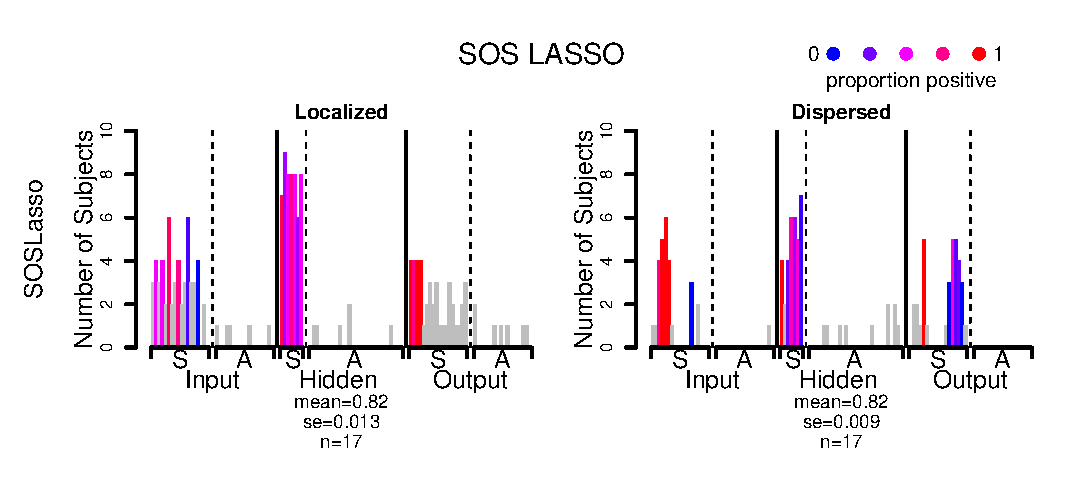
\includegraphics[width=0.95\textwidth]{figures/figure9.eps}
\caption{The results from the {\soslasso} analysis. The height of each bar corresponds to the number of times each unit was selected over subjects. Colored bars were selected more times than would be expected given the overall rate of unit selection. The blueness or redness of the bar conveys the frequency with which each unit was assigned a positive weight over subjects. Positive weights mean that activation at that unit will push the model towards labeling the current item as belonging to domain A. Mean and se indicate the mean and standard error of the classifier accuracy, respectively; n indicates the number of units selected more often than chance across model subjects.}
\label{fig.sos} 
\end{figure}

The first point of note is that the {\soslasso} classifier showed a mean cross-validation accuracy across subjects of 0.82 in both the localized and anatomically dispersed model variants---much higher than searchlight, {\lasso}, and ridge regression, all of which showed accuracies between 0.6--0.65. This stark difference suggests that {\soslasso} is able to exploit cross-subject consistency in the location of useful units to better find the informative signal in individual models.

Figure \ref{fig.sos} shows, for each unit, how frequently it was identified as important across model individuals. As with {\lasso}, the base-rate of unit selection was used to conduct a binomial test across model individuals, to indicate which units were selected more often than expected by chance. The method clearly excels at identifying the SH units. When these are localized, all units are reliably identified, but even when they are anatomically dispersed, the method reliably finds 6 of the 7 units. Arbitrary units are almost never flagged as important for representation. Compared to {\lasso}, the method also does a slightly better job identifying the systematic I/O units, reliably identifying 11 of the 36 units (31\%) in both cases.

The rightmost panel of Figure \ref{fig.precision} shows the mean precision and hit rate across individuals in the anatomically localized and dispersed models. Considering all units, {\soslasso} maintains the same precision as {\lasso}, but with a substantially better hit rate. With localized representations, this improvement was observed for both hidden and I/O units. When hidden representations were anatomically dispersed, the precision declined slightly but the hit rate still improved markedly. In the dispersed case the precision declines when the method sometimes selects arbitrary units belonging to groups containing signal-carrying units. An arbitrary unit contained in a selected set and happening to spuriously covary with the class label may itself be selected. Despite such inclusions, however, the overall gain in hit rate with minimal loss of precision, together with the greatly improved classifier cross-validation accuracy, suggest that {\soslasso} is doing a substantially better job of finding useful representational structure.

The advantages of {\soslasso} are clear when representations are anatomically localized, but what accounts for the improved hit rate when they are dispersed? The first observation is that, though signal-carrying voxels do not line up across subjects, there exist some sets that happen to contain many signal-carrying voxels across subjects, while others contain mostly arbitrary voxels. Because selecting voxels from many sets is more expensive than selecting the same number of voxels from fewer sets, {\soslasso} strives to select voxels from the smallest number of sets possible. If this were the only reason, however, then the searchlight method should have also succeeded. The second observation is that all of the selected voxels across groups contribute to a single classifier, just as in {\lasso} and ridge regression. Thus {\soslasso} can perform well even when the useful information is distributed over multiple sets. In general {\soslasso} builds the best sparse whole-brain classifier possible while keeping solutions for different subjects as similar as possible, where similarity is defined by membership in the same set.

It is worth noting here that the {\soslasso} is a generalized optimization within which {\lasso} itself is a special case. As noted earlier, when the parameter controlling the weight on the group sparsity penalty is set to zero, the regularizer reduces to the standard {\lasso} penalty. This means that the parameterization of {\soslasso} itself indicates the extent to which there exists useful cross-subject consistency in signal location. If no such consistency exists, the classifier cross-validation accuracy will not exceed that of {\lasso} alone, and the best estimate for the group-sparsity parameter will be near zero. For real data, this suggests a way of testing whether there exists cross-subject consistency in information localization. The {\soslasso} classifier will only perform better than the {\lasso} classifier if such consistency exists.

Finally, with regard to laying bare the representational code, {\soslasso} performs similarly to {\lasso}: Where units are reliably discovered, the nature of the code is clear from the weight values (colored bars in Figure \ref{fig.sos}), though these patterns are somewhat noisy when the units are only discovered in a small number of model individuals.

These results provide answers to our core questions, summarized in Table \ref{tab.modelresults}.

\begin{table}
	\begin{tabular}{L{.25\textwidth} c c c c c}
\toprule
Result         & Univariate  & Searchlight& {\lasso}      & Ridge      & {\soslasso}  \\
\midrule
\ModResults{1} &  \checkmark & \checkmark$^\dagger$ &            & \checkmark$^\ddagger$ & \checkmark \\
\ModResults{2} &             & \checkmark$^\dagger$ & \checkmark & \checkmark$^\ddagger$ & \checkmark \\
\ModResults{3} &  \checkmark &            & \checkmark & \checkmark$^\ddagger$ & \checkmark \\
\ModResults{4} &  \checkmark & \checkmark &            &            &            \\
\bottomrule
\end{tabular}

%%% table_results_content.tex: 
%\newcommand{\ModResults}[1]{
% \switch[#1]
%  \case{=1} Identifies SI/O units %
%  \case{=2} Identifies HI/O units %
%  \case{=3} Indicates unit-level contributions %
%  \case{=4} Requires localized representation %
% \endswitch  	
%}




%\begin{tabular}{l c c c c c c c}
%\toprule
% &\multicolumn{2}{c}{Identifies}& &\\
% \cmidrule{2-3}
% & SI/O & SH & Indicates & Needs Local \\
% \midrule
%UC & \checkmark & & \checkmark & \checkmark \\
%SL & \checkmark & \checkmark & & \checkmark \\
%R & \checkmark$^*$ & \checkmark$^*$ & \checkmark$^*$ & \\
%L & & \checkmark & \checkmark & \\
%SOS & \checkmark & \checkmark & \checkmark & \\
%\bottomrule
%\end{tabular}
	\caption{A summary of the answers for each method across the four central questions. $\dagger$ The success of the searchlight was contingent on model parameters that may be difficult to discern in practice. $\ddagger$ Ridge regression identifies all units as informative, including ones that in fact contain no information.} 
	\label{tab.modelresults}
\end{table}

\begin{center}
	\textbf{--- Table \ref{tab.modelresults} about here---}
\end{center}

%In sum, {\soslasso} shows the following answers to the core questions: 
%
%\begin{enumerate}
%\item {\bf Does the method reliably identify the systematic I/O units?} It does so better than LASSO, but not as well as searchlight or univariate analysis. The method assumes an overall sparse representation, and so will find a small set of units that strongly encode the information of interest. Where signal is weakly coded across many redundant units, {\soslasso} will still tend to miss many units.
%\item {\bf Does the method reliably identify the systematic hidden units?} Yes---of all methods, {\soslasso} has the highest hit rate and precision for the SH units, in both localized and dispersed cases.
%\item {\bf Does the method indicate how the information of interest is coded across identified units?} Like LASSO, it does so quite well for identified units.
%\item {\bf Do method results depend on anatomical localization of signal-carrying units?} Somewhat: The method had slightly lower precision and hit rates among hidden units when these were anatomically dispersed, though the effects were much milder than those observed for searchlight.
%\end{enumerate}
%
